\documentclass[a4paper,openright,12pt,oneside]{article}
\usepackage[top=2cm, bottom=2cm, left=2.5cm, right=2.5cm]{geometry}
\usepackage{graphicx} % Required for inserting 
\usepackage{float}
\usepackage[dvipsnames]{xcolor}
\usepackage{emoji}
\usepackage{setspace}\usepackage[siunitx]{circuitikz}
\usetikzlibrary{positioning, arrows.meta}
\usepackage[utf8]{inputenc}
\usepackage[spanish]{babel}
\usepackage{amsmath}
\usepackage{booktabs}
\usepackage[utf8]{inputenc}
\usepackage[x11names]{xcolor}
\usepackage{tcolorbox}
\usepackage{fontspec}


\newtcolorbox{terminal}{
  colback=gray!15!black,
  colframe=gray!15!black,
  arc=0pt,
  outer arc=0pt,
  left=2pt,
  right=2pt,
  top=2pt,
  bottom=2pt,
  boxrule=0pt
}

\newcommand{\promptA}{\textcolor{green!70!black}{Said@DESKTOP-H8DC8IG} \textcolor{magenta!80!white}{MINGW64} \textcolor{yellow!80!white}{\textasciitilde/codigo mal hecho} \textcolor{cyan!80!white}{(ramatototota)}\\ \textcolor{white}{\$ }}

\newcommand{\promptB}{\textcolor{green!70!black}{Said@DESKTOP-H8DC8IG} \textcolor{magenta!80!white}{MINGW64} \textcolor{yellow!80!white}{\textasciitilde/codigo mal hecho/reporprueba1} \textcolor{cyan!80!white}{(main)}\\ \textcolor{white}{\$ }}

\newcommand{\promptC}{\textcolor{green!70!black}{Said@DESKTOP-H8DC8IG} \textcolor{magenta!80!white}{MINGW64} \textcolor{yellow!80!white}{\textasciitilde/codigo mal hecho/reporprueba1/Software ultra secreto} \textcolor{cyan!80!white}{(main)}\\ \textcolor{white}{\$ }}

\newcommand{\prompt}{\textcolor{green!70!black}{dorian@dorian-HP-Pavilion-Laptop-15-eh3xxx}:\textcolor{cyan!80!white}{\textasciitilde/UV/olmedo/reporprueba1\$ }}

\newcommand{\promptD}{\textcolor{green!70!black}{Said@DESKTOP-H8DC8IG} \textcolor{magenta!80!white}{MINGW64} \textcolor{yellow!80!white}{\textasciitilde/codigo mal hecho/reporprueba1/Software ultra secreto} \textcolor{cyan!80!white}{(main)}\\ \textcolor{white}{\$ }}

\usetikzlibrary{positioning, arrows.meta, calc}

\title{Act.Indiviual. Ciclo for en python}
\author{Felipe de Jesús Montaño Rocha}
\definecolor{azul}{RGB}{0,51,153}


\title{Reporte de prácticas \#} %O reporte de simulacion

\begin{document}
\begin{titlepage} %Aquí modificar los datos necesarios
\begin{center}
   {\Huge \textbf{Universidad Veracruzana \vspace{1cm}\\}}
   
   
\includegraphics[width=0.4\textwidth]{imagenes/LOGO.jpg}~\\[1cm]
   
   {\LARGE \textbf{Facultad de Ingeniería en Electrónica y Comunicaciones}}\\
   \vspace{0.4cm}
   {\Large Reporte de Actividad \\\vspace{0.4cm} \textbf{Documentación de proyectos en Tecnologías Computacionales}}
   \vspace{0.3cm}
   \textcolor{azul}{\rule{\linewidth}{0.75mm}}\\
   \begin{spacing}{1.0}
 
   {\LARGE \textsc{Actividad en equipo: \\\vspace{0.2cm} Git Issues}}
   \end{spacing}
   \textcolor{azul}{\rule{\linewidth}{0.75mm}}\\
   \vspace{0.6cm}
   {\Large \textbf{Alumno:}}\\

  {\Large
\begin{center} 
   Dorian Emir Cardenas Vicente S24006903 \\
   Bryan Guerrero Cruz S24006895\\
   Luis Said Hernández Rodríguez S24006917\\
   Felipe de Jesus Montaño Rocha S24006886
   
\end{center}
}
    \vspace{0.1cm}
    {\Large \textbf{Docente:}}\\
   \vspace{0.1cm}
   {\Large M. Sc. Luis Fernando Olmedo García}
   \vfill
   
   {\LARGE \textbf{Junio 02, 2026} \\\vspace{0.3cm} }%aqui esta la fecha 
\end{center}
\end{titlepage}


\section{Introducción}
En esta actividad aprendimos a usar y utilizamos los ''Issues'', estos mismos son herramientas de GitHub nos permite realizar varias acciones, cuales como reportar errores que puede generar un código mal implementado por nuestros colaboradores, también nos permite agregar tareas nuevas a los repositorios en donde nos encontremos trabajando, dentro de un ambiente colaborativo, al igual que podemos realizar la petición de la mejora de algún código incompleto o que puede llegar a complementarse a un mejor proyecto de software, otra de sus funciones más representativas es la posibilidad de crear una buena organización en un equipo para la realización de un trabajo colaborativo con el fin de realizar un proyecto.
\\En esta practica se realizó la creación de un Issue desde dos maneras posibles la primera fue la creación un Issue por medio de una pagina web y la segunda forma fue crear un Issue desde la terminal de VS code, las dos maneras de realizar esta actividad tienen su propia forma de realización, sus comandos aplicables, cada miembro del equipo participo en la creación de los Issues en las dos formas descritas en el documento de la actividad propuesta.




\section{Crear un issue desde la página web}

Para crear un issue desde la página web de GitHub, primero me uní a un repositorio colaborativo. Una vez en dentro del repositorio, debemos de dirigirnos a la pesaña de issues y luego damos clic en nuevooo issue "New issue". Ahora, agregamos una descripción, un título al issue, podemos agregar una etiqueta (aparecen en la parte de la derecha y dice "label") dependiendo para que caso.

\begin{figure}[H]
    \centering
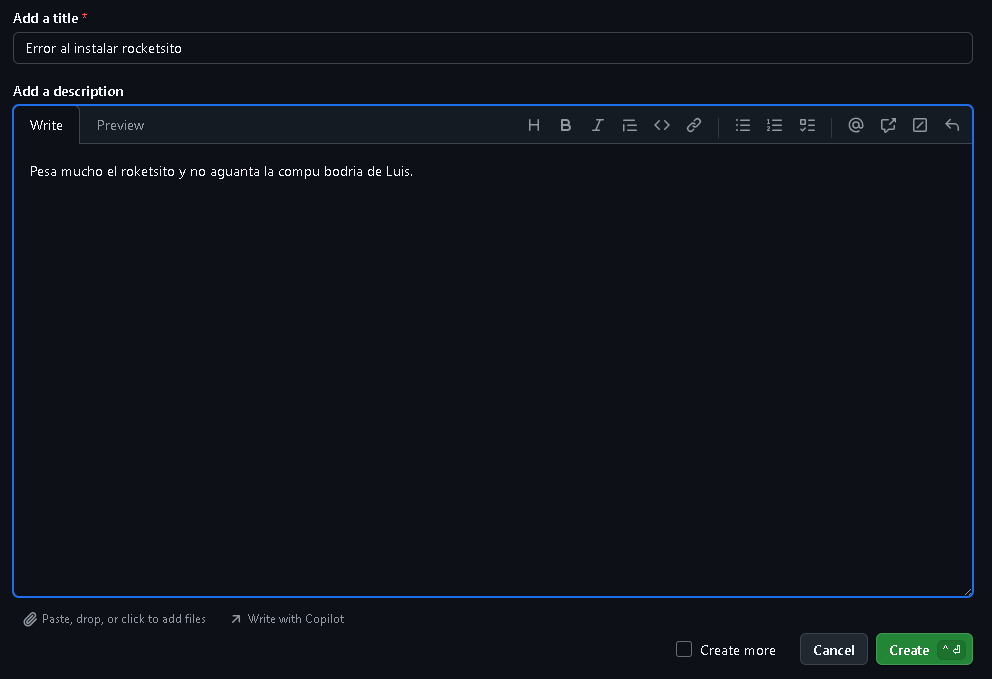
\includegraphics[width=1\textwidth]{imagenes/img/issue1.png}
    \caption{Creación de un issue desde la página web}
    \label{fig:D1}
\end{figure}

\begin{figure}[H]
    \centering
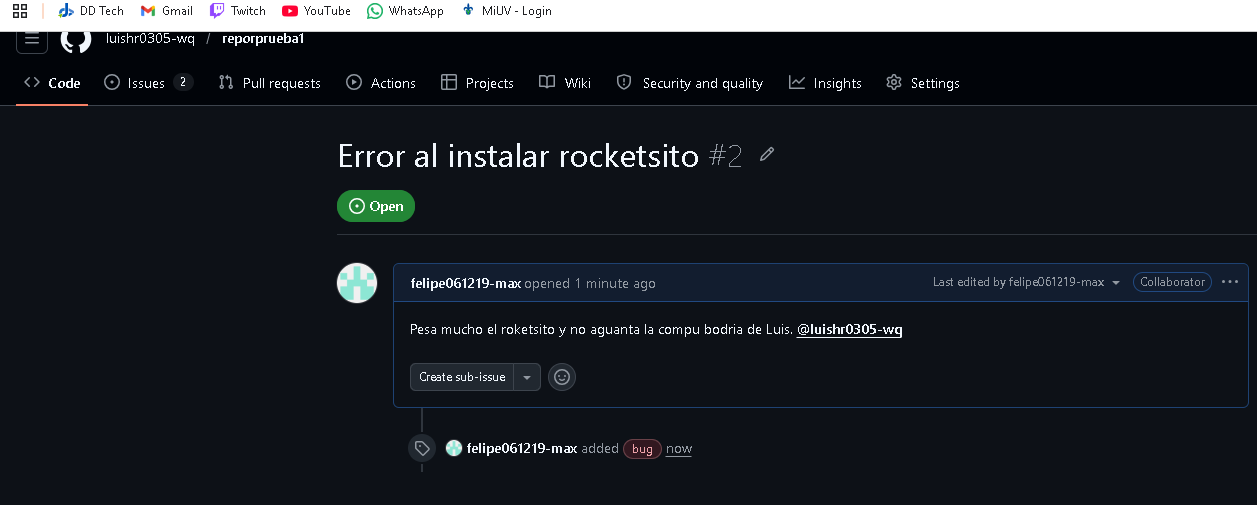
\includegraphics[width=1\textwidth]{imagenes/img/issue2.png}
    \caption{Agregar etiquetas}
    \label{fig:D2}
\end{figure}

Aquí ya podemos visualizar los issues abiertos y cerrados del repositorio, así como la etiqueta del issue y el responsable.

\begin{figure}[H]
    \centering
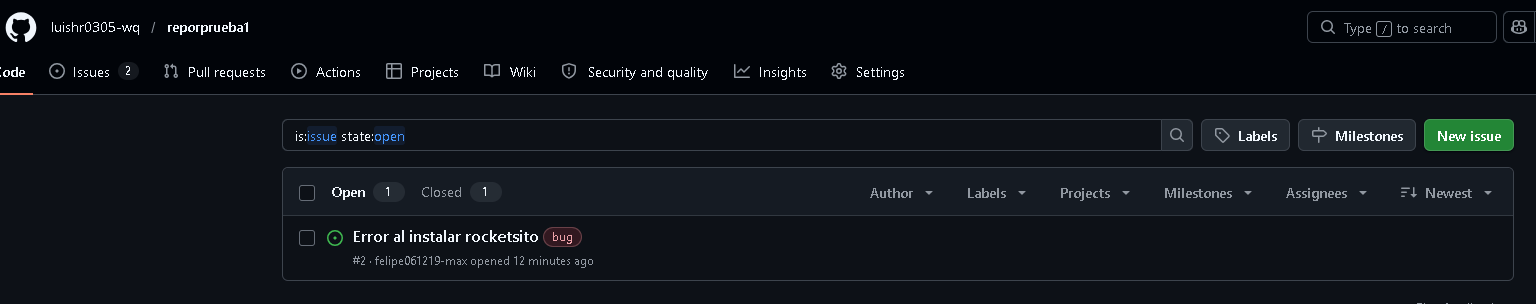
\includegraphics[width=1\textwidth]{imagenes/img/issue3.png}
    \caption{Visualización del issue en el repositorio}
    \label{fig:D3}
\end{figure}

\begin{figure}[H]
    \centering
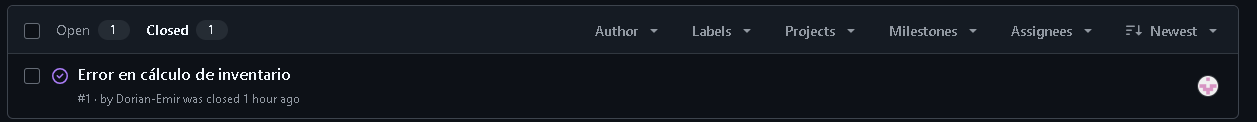
\includegraphics[width=1\textwidth]{imagenes/img/issue_c.png}
    \caption{Visualización del issue en el repositorio}
    \label{fig:D4}
\end{figure}

\end{document}